\documentclass[../main.tex]{subfiles}
\begin{document}
\chapter{2016-2017学年微积分（一）（下）期末考试}

\section{单项选择题(每小题 3 分，共 18 分)}
\begin{enumerate}
    \item 考虑二元函数$f(x,y)$在点$(x_{0},y_{0})$处的下面四条性质：

          （1）连续；（2）两个偏导数存在；（3）可微；（4）沿方向$(1,0)$的方向导数存在.

          若用“$P\Rightarrow Q$”表示可由性质$P$推出性质$Q$，则成立（\qquad）.

          \begin{tasks}[label=\textbf{\Alph*.}, label-width=1.5em, column-sep=1em](2)
              \task $(2)\Rightarrow(3)\Rightarrow(1)$
              \task $(3)\Rightarrow(2)\Rightarrow(1)$
              \task $(3)\Rightarrow(4)\Rightarrow(1)$
              \task $(3)\Rightarrow(2)\Rightarrow(4)$
          \end{tasks}

    \item 将$I=\int_{0}^{1}\,\mathrm{d}y\int_{-y}^{y}f(x,y)\,\mathrm{d}x$化为先对$y$后对$x$的逐次积分，正确结果是（\qquad）.

          \begin{tasks}[label=\textbf{\Alph*.}, label-width=1.5em, column-sep=1em](1)
              \task $\displaystyle I=\int_{-1}^{0}\,\mathrm{d}x\int_{x}^{1}f(x,y)\,\mathrm{d}y+\int_{0}^{1}\,\mathrm{d}x\int_{-x}^{1}f(x,y)\,\mathrm{d}y$
              \task $\displaystyle I=\int_{-y}^{y}\,\mathrm{d}x\int_{0}^{1}f(x,y)\,\mathrm{d}y$
              \task $\displaystyle I=\int_{-1}^{0}\,\mathrm{d}x\int_{-x}^{1}f(x,y)\,\mathrm{d}y+\int_{0}^{1}\,\mathrm{d}x\int_{x}^{1}f(x,y)\,\mathrm{d}y$
              \task $\displaystyle I=\int_{0}^{1}\,\mathrm{d}x\int_{-x}^{x}f(x,y)\,\mathrm{d}y$
          \end{tasks}

    \item 设$L$表示圆$x^{2}+y^{2}=R^{2}(R>0)$，取顺时针方向，则积分$\oint_{L}-x^2y\,\mathrm{d}x+xy^2\,\mathrm{d}y=\text{（\qquad）}$.

          \begin{tasks}[label=\textbf{\Alph*.}, label-width=1.5em, column-sep=1em](2)
              \task $\pi R^{4}$
              \task $-\dfrac{\pi R^{4}}{2}$
              \task $-\pi R^{4}$
              \task $\dfrac{\pi R^{4}}{2}$
          \end{tasks}

    \item 设$a_{n}>0(n=1,2,\cdots)$，下列说法中正确的是（\qquad）.

          \begin{tasks}[label=\textbf{\Alph*.}, label-width=1.5em, column-sep=1em](1)
              \task 若级数$\sum\limits_{n=1}^{\infty}(-1)^{n}a_{n}$条件收敛，则级数$\sum\limits_{n=1}^{\infty}a_{2n}$发散
              \task 若级数$\sum\limits_{n=1}^{\infty}(-1)^{n}a_{n}$绝对收敛，则级数$\sum\limits_{n=1}^{\infty}a_{2n}$发散
              \task 若级数$\sum\limits_{n=1}^{\infty}a_{n}$收敛，则级数$\sum\limits_{n=1}^{\infty}(-1)^{n}a_{n}$条件收敛
              \task 若级数$\sum\limits_{n=1}^{\infty}a_{n}$发散，则当$n$充分大时，$a_{n}\geq \dfrac1n$
          \end{tasks}

    \item 二阶常系数线性微分方程$y''-3y'-4y=x+\mathrm{e}^{-x}$的特解的待定形式为（\qquad）.

          \begin{tasks}[label=\textbf{\Alph*.}, label-width=1.5em, column-sep=1em](2)
              \task $y^{*}=ax+b+c\mathrm{e}^{-x}$
              \task $y^{*}=x(ax+b)+(cx+d)\mathrm{e}^{-x}$
              \task $y^{*}=ax+b+c x\mathrm{e}^{-x}$
              \task $y^{*}=x(ax+b)+c x\mathrm{e}^{-x}$
          \end{tasks}

    \item 设$\sum\limits_{n=1}^{\infty}b_{n}\sin nx$是将函数$f(x)=x+1(0\leq x\leq\pi)$做奇延拓后展开成的傅立叶级数，其和函数为$S(x)(-\infty<x<+\infty)$，则$S\left(-\frac{5\pi}{2}\right)=\text{（\qquad）}$.

          \begin{tasks}[label=\textbf{\Alph*.}, label-width=1.5em, column-sep=1em](2)
              \task $-\dfrac{\pi}{2}+1$
              \task $\dfrac{\pi}{2}+1$
              \task $-\dfrac{\pi}{2}-1$
              \task $\dfrac{\pi}{2}-1$
          \end{tasks}
\end{enumerate}

\section{填空题(每小题 4 分，共 16 分)}
\begin{enumerate}
    \setcounter{enumi}{6}
    \item 设函数$z=x\mathrm{e}^{y}$，则$\mathrm{d}z\Big|_{\substack{x=0 \\ y=1}}=$\underline{\hspace{3cm}}.

    \item 设$D:x^{2}+y^{2}\leq1,\ y\geq0$，则$\iint\limits_{D}\bigl[(x+1)^{2}+y^{2}\bigr]\mathrm{d}x\,\mathrm{d}y=\underline{\hspace{3cm}}$.

    \item 设$L$是圆周$x^{2}+y^{2}=1$，则$\oint_{L}(x^2+xy)\,\mathrm{d}s=\underline{\hspace{3cm}}$.

    \item 设曲面$S=\{(x,y,z):z=1,|x|\leq1,|y|\leq1\}$，则$\iint\limits_{S}(x+y+z)\,\mathrm{d}S=\underline{\hspace{3cm}}$.
\end{enumerate}

\section{基本计算题(每小题 7 分，共 42 分)}
\begin{enumerate}
    \setcounter{enumi}{10}
    \item 求经过直线$
              L:\begin{cases}
                  2x+3y-z-8=0, \\
                  y-3z+4=0
              \end{cases}$
          且与平面$\pi:x+y+z-4=0$平行的平面方程$\pi_{1}$.
          \vspace{11em}

    \item 设$z=f(\mathrm{e}^{2x},xy)$，其中$f$具有二阶连续导数，且$f_{2}'(1,0)=2$，求$\left.\frac{\partial^{2}z}{\partial x\partial y}\right|_{\substack{x=0\\y=3}}$.
          \vspace{8em}

    \item 设变量$x,y,t$满足方程$x=F(t,y)$和$f(x+y+t)=3y$，其中$f$具有一阶连续导数，$F$具有一阶连续偏导数，记$F_{1}=\frac{\partial F(t,y)}{\partial t}$，$F_{2}=\frac{\partial F(t,y)}{\partial y}$，
          且$1+F_{1}\neq0,\ f'\neq0$，求$\dfrac{\mathrm{d}x}{\mathrm{d}y}$.
          \vspace{8em}

    \item 设$L$是依逆时针方向的下半圆周$x^{2}+y^{2}=x\ (y\leq0)$，求曲线积分
          \[
              I=\int_{L}(1-y-\mathrm{e}^{x}\sin y)\,\mathrm{d}x+(1-\mathrm{e}^{x}\cos y)\,\mathrm{d}y.
          \]
          \vspace{8em}

    \item 设$S$为曲面$z=-\sqrt{1-x^{2}-y^{2}}$的上侧，求曲面积分
          \[
              I=\iint\limits_{S}xyz\,\mathrm{d}y\,\mathrm{d}z+x^{2}y\,\mathrm{d}z\,\mathrm{d}x+\left(\frac{z^{3}}{3}+1\right)\,\mathrm{d}x\,\mathrm{d}y.
          \]
          \vspace{8em}

    \item 将$f(x)=\arctan\dfrac{1+x}{1-x}$展成$x$的幂级数.
          \vspace{9em}
\end{enumerate}

\section{应用题(每小题 7 分，共 14 分)}
\begin{enumerate}
    \setcounter{enumi}{16}
    \item 求函数$f(x,y,z)=xy+z^{2}$在平面$x=y$与球面$x^{2}+y^{2}+z^{2}=4$相交的圆周上的最大值和最小值.
          \vspace{10em}

    \item 设函数$\varphi(x)$具有连续的一阶导数，且满足$\varphi(0)=0$，$\varphi'(x)+\int_{0}^{x}\varphi(t)\,\mathrm{d}t=\mathrm{e}^{x}$，求$\varphi(x)$.
          \vspace{10em}
\end{enumerate}

\section{分析证明题(每小题 5 分，共 10 分)}
\begin{enumerate}
    \setcounter{enumi}{18}
    \item 讨论级数
          \[
              \sum_{n=1}^{\infty}\left[1-\sin\left(\frac{(-1)^{n}}{n^{p}}\right)-\cos\left(\frac{(-1)^{n}}{n^{p}}\right)\right]\qquad (p>0)
          \]
          的敛散性，收敛时指明是条件收敛还是绝对收敛.
          \vspace{10em}

    \item 设函数$f(x)$在区间$[a,b](a>0)$上连续，且$f(x)>0$，证明：
          \[
              \int_{a}^{b}xf(x)\,\mathrm{d}x\int_{a}^{b}\frac{x}{f(x)}\,\mathrm{d}x\geq\frac{(b+a)^2(b-a)^2}{4}.
          \]
          \vspace{10em}
\end{enumerate}

\chapter{2016-2017学年微积分（一）（下）期末考试参考答案}
\section{单项选择题(每小题 3 分，共 18 分)}
\begin{enumerate}
    \item \textbf{Solution}. D.

          可微必推出两个偏导数存在，而偏导数是特殊方向的方向导数. 由于方向 $(1,0)$ 即为 $x$ 轴正方向，

          故偏导数存在可直接推出该方向导数存在，因此$(3)\Rightarrow(2)\Rightarrow(4)$成立.

    \item \textbf{Solution}. C.

          \noindent
          \begin{minipage}[c]{0.65\textwidth}
              如图，积分区域为
              \[
                  D=\{(x,y):0\le y\le1,\ -y\le x\le y\}.
              \]
              改为先对$y$积分时，$-1\le x\le1$，且当$-1\le x\le0$时，$-x\le y\le1$；

              当$0\le x\le1$时，$x\le y\le1$.
          \end{minipage}
          \hfill %
          \begin{minipage}[c]{0.36\textwidth}
              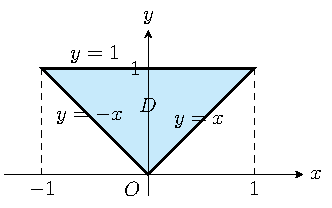
\includegraphics[width=4.8cm]{2017xf-figure1.pdf}
          \end{minipage}

          故
          \[
              I=\int_{-1}^{0}\,\mathrm{d}x\int_{-x}^{1}f(x,y)\,\mathrm{d}y+
              \int_{0}^{1}\,\mathrm{d}x\int_{x}^{1}f(x,y)\,\mathrm{d}y.
          \]

    \item \textbf{Solution}. B.

          记$P=-x^2y,\ Q=xy^2$. 若$L$取逆时针方向，则由Green公式，
          \[
              \oint_L P\,\mathrm{d}x+Q\,\mathrm{d}y
              =\iint\limits_{x^2+y^2\le R^2}(Q_x-P_y)\,\mathrm{d}x\,\mathrm{d}y
              =\iint\limits_{x^2+y^2\le R^2}(x^2+y^2)\,\mathrm{d}x\,\mathrm{d}y
              =\frac{\pi R^4}{2}.
          \]
          题中为顺时针方向，所以积分值为$-\dfrac{\pi R^4}{2}$.

    \item \textbf{Solution}. A.

          对于A，B选项，记级数的前$2N$项部分和为$S_{2N}$，绝对值级数的前$2N$项部分和为$T_{2N}$，则
          \[
              \begin{aligned}
                  S_{2N}+T_{2N}= {} & \left(-a_1+a_2-a_3+a_4-\cdots -a_{2N-1}+a_{2N}\right)+\left(a_1+a_2+a_3+a_4+\cdots +a_{2N-1}+a_{2N}\right) \\
                  ={}               & 2\sum_{n=1}^{N}a_{2n}.
              \end{aligned}
          \]
          若$\sum(-1)^na_n$条件收敛，则$S_{2N}$收敛，但$T_{2N}$发散，所以$\sum a_{2n}$发散.

          若$\sum(-1)^na_n$绝对收敛，则$S_{2N}$和$T_{2N}$都收敛，所以$\sum a_{2n}$收敛.

          对于C选项，令$a_n=\frac{1}{n^2}$，则$\sum a_n$收敛，且$\sum(-1)^na_n=\sum \frac{(-1)^n}{n^2}$绝对收敛.

          对于D选项，令$a_n=\begin{cases}
                  1,             & n=2k,  \\
                  \frac{1}{n^2}, & n=2k-1
              \end{cases}$，则$\sum a_n$发散，但当$n$充分大且为奇数时，$a_n<\frac{1}{n}$.

    \item \textbf{Solution}. C.

          方程对应齐次方程的特征方程为
          \[
              r^2-3r-4=(r-4)(r+1)=0.
          \]
          所以齐次方程的通解为$y_h=C_1\mathrm{e}^{4x}+C_2\mathrm{e}^{-x}$.

          对于非齐次项$y_1=x$，由于$\lambda=0$不是齐次方程的根，所以特解为$y_1^*=ax+b$；

          对于非齐次项$y_2=\mathrm{e}^{-x}$，由于$\lambda=-1$是齐次方程的单根，所以特解为$y_2^*=cx\mathrm{e}^{-x}$.

          由解的叠加原理，特解的待定形式为$y^*=y_1^*+y_2^*=ax+b+cx\mathrm{e}^{-x}$.

    \item \textbf{Solution}. C.

          奇延拓后的和函数是以$2\pi$为周期的奇函数. 因此
          \[
              S\left(-\frac{5\pi}{2}\right)=S\left(-\frac{\pi}{2}\right)
              =-f\left(\frac{\pi}{2}\right)
              =-\frac{\pi}{2}-1.
          \]

\end{enumerate}

\section{填空题(每小题 4 分，共 16 分)}
\begin{enumerate}
    \setcounter{enumi}{6}
    \item \textbf{Solution}. $\mathrm{e}\,\mathrm{d}x$.

          因为
          \[
              \mathrm{d}z=\mathrm{e}^y\,\mathrm{d}x+x\mathrm{e}^y\,\mathrm{d}y,
          \]
          所以$\mathrm{d}z\Big|_{\substack{x=0 \\ y=1}}=\mathrm{e}\,\mathrm{d}x$.

    \item \textbf{Solution}. $\dfrac{3\pi}{4}$.

          在上半圆盘$D$上，由对称性可知$\iint\limits_D2x\,\mathrm{d}x\,\mathrm{d}y=0$. 因此
          \[
              \begin{aligned}
                  \iint\limits_D\bigl[(x+1)^2+y^2\bigr]\,\mathrm{d}x\,\mathrm{d}y={} & \iint\limits_D(x^2+y^2)\,\mathrm{d}x\,\mathrm{d}y+\iint\limits_D\,\mathrm{d}x\,\mathrm{d}y \\
                  ={}                                                                & \pi\int_{0}^{1}r^3\,\mathrm{d}r+\frac{\pi}{2}=\frac{3\pi}{4}.
              \end{aligned}
          \]

    \item \textbf{Solution}. $\pi$.

          令$x=\cos t,\ y=\sin t\ (0\le t\le2\pi)$，则$\mathrm{d}s=\mathrm{d}t$. 因而
          \[
              \oint_L(x^2+xy)\,\mathrm{d}s
              =\int_0^{2\pi}(\cos^2t+\cos t\sin t)\,\mathrm{d}t=\pi.
          \]

    \item \textbf{Solution}. $4$.

          曲面为平面方形区域，$\mathrm{d}S=\mathrm{d}x\,\mathrm{d}y$，故由对称性可知
          \[
              \begin{aligned}
                  \iint\limits_S(x+y+z)\,\mathrm{d}S={} & \iint\limits_{\substack{-1\le x\le1 \\ -1\le y\le1}}(x+y+1)\,\mathrm{d}x\,\mathrm{d}y \\
                  ={}                                   & \iint\limits_{\substack{-1\le x\le1 \\ -1\le y\le1}}\,\mathrm{d}x\,\mathrm{d}y=4.
              \end{aligned}
          \]

\end{enumerate}

\section{基本计算题(每小题 7 分，共 42 分)}
\begin{enumerate}
    \setcounter{enumi}{10}
    \item \textbf{Solution}. 因$\pi_1$与$\pi:x+y+z-4=0$平行，可设
          \[
              \pi_1:x+y+z+D=0.
          \]
          在方程组中令$z=0$，可取直线$L$上一点$P(10,-4,0)$，代入得$D=-6$，故
          \[
              \pi_1:x+y+z-6=0.
          \]

    \item \textbf{Solution}. 先求
          \[
              z_x=2\mathrm{e}^{2x}f_1'(\mathrm{e}^{2x},xy)+yf_2'(\mathrm{e}^{2x},xy).
          \]
          令
          \[
              G(x,y)=2\mathrm{e}^{2x}f_1'(\mathrm{e}^{2x},xy)+yf_2'(\mathrm{e}^{2x},xy),
          \]
          则$G(0,y)=2f_1'(1,0)+yf_2'(1,0)=2f_1'(1,0)+2y$，$G_y(0,y)=f_2'(1,0)\equiv2$，因而
          \[
              \left.\frac{\partial^{2}z}{\partial x\partial y}\right|_{\substack{x=0\\y=3}}=G_y(0,3)=2.
          \]

    \item \textbf{Solution}. 由
          \[
              \begin{cases}
                  x=F(t,y), \\
                  f(x+y+t)=3y
              \end{cases}
          \]
          确定$t=t(y),\ x=x(y)$. 两边对$y$求导，得
          \[
              \begin{cases}
                  x'=F_1t'+F_2, \\
                  (x'+t'+1)f'=3.
              \end{cases}
          \]
          解得
          \[
              \frac{\mathrm{d}x}{\mathrm{d}y}=\frac{f'F_2+(3-f')F_1}{(1+F_1)f'}.
          \]

    \item \textbf{Solution}. 补线段$L_1:y=0,\ x:1\to0$，则$L+L_1$封闭并取正向. 故
          \[
              I=\oint_{L+L_1}(1-y-\mathrm{e}^x\sin y)\,\mathrm{d}x+(1-\mathrm{e}^x\cos y)\,\mathrm{d}y-
              \int_{L_1}\,\mathrm{d}x.
          \]
          由Green公式，记$D:\{(x,y)|x^2+y^2\le x, y\leq 0\}$，则
          \[
              \begin{aligned}
                  I={} & \oint_{L+L_1}(1-y-\mathrm{e}^x\sin y)\,\mathrm{d}x+(1-\mathrm{e}^x\cos y)\,\mathrm{d}y-\int_{1}^{0}\,\mathrm{d}x \\
                  ={}  & \iint\limits_{D}\left[-\mathrm{e}^x\cos y-\left(-1-\mathrm{e}^x\cos y\right)\right]\,\mathrm{d}x\,\mathrm{d}y+1  \\
                  ={}  & \iint\limits_{D}\,\mathrm{d}x\,\mathrm{d}y+1=\frac{\pi}{8}+1.
              \end{aligned}
          \]

    \item \textbf{Solution}. 记底面$S_1:z=0,\ x^2+y^2\le1$取下侧，区域$\Sigma:\{(x,y,z)|x^2+y^2+z^2\le1, z\le0\}$，

          则$S+S_1$封闭并指向内侧. 所以由Gauss公式可知
          \[
              \begin{aligned}
                  I={} & \oiint\limits_{S+S_1}xyz\,\mathrm{d}y\,\mathrm{d}z+x^{2}y\,\mathrm{d}z\,\mathrm{d}x+\left(\frac{z^{3}}{3}+1\right)\,\mathrm{d}x\,\mathrm{d}y-\iint\limits_{S_1}\left(\frac{z^{3}}{3}+1\right)\,\mathrm{d}x\,\mathrm{d}y \\
                  ={}  & -\iiint\limits_{\Sigma} \left(yz+x^2+z^2\right)\,\mathrm{d}x\,\mathrm{d}y\,\mathrm{d}z+\iint\limits_{x^2+y^2\le1}\,\mathrm{d}x\,\mathrm{d}y                                                                             \\
                  ={}  & -\iiint\limits_{\Sigma} \left(yz+x^2+z^2\right)\,\mathrm{d}x\,\mathrm{d}y\,\mathrm{d}z+ \pi.
              \end{aligned}
          \]

          由对称性可知$\iiint\limits_{\Sigma}yz\,\mathrm{d}x\,\mathrm{d}y\,\mathrm{d}z=0$，$\iiint\limits_{\Sigma}x^2\,\mathrm{d}x\,\mathrm{d}y\,\mathrm{d}z=\iiint\limits_{\Sigma}y^2\,\mathrm{d}x\,\mathrm{d}y\,\mathrm{d}z=\iiint\limits_{\Sigma}z^2\,\mathrm{d}x\,\mathrm{d}y\,\mathrm{d}z$.

          因此
          \[
              \begin{aligned}
                  I={} & -\frac{2}{3}\iiint\limits_{\Sigma}\left(x^2+y^2+z^2\right)\,\mathrm{d}x\,\mathrm{d}y\,\mathrm{d}z+\pi                               \\
                  ={}  & -\frac{2}{3}\int_{0}^{2\pi}\,\mathrm{d}\theta\int_{0}^{\frac{\pi}{2}}\sin\varphi\,\mathrm{d}\varphi\int_{0}^{1}r^4\,\mathrm{d}r+\pi \\
                  ={}  & -\frac{2}{3}\cdot 2\pi\cdot \frac{1}{5}+\pi=\frac{11\pi}{15}.
              \end{aligned}
          \]

    \item \textbf{Solution}. 注意到
          \[
              f'(x)=\frac{1}{1+x^2}=\sum_{n=0}^{\infty}(-1)^nx^{2n},\qquad |x|<1,
          \]
          上式两端从$0$积分到$x$，并利用$f(0)=\dfrac{\pi}{4}$，得
          \[
              f(x)-\frac{\pi}{4}=\sum_{n=0}^{\infty}\int_{0}^{x}(-1)^nt^{2n}\,\mathrm{d}t=\sum_{n=0}^{\infty}\frac{(-1)^nx^{2n+1}}{2n+1},\qquad |x|<1.
          \]

          又当$x=1$时，级数$\sum_{n=0}^{\infty}\frac{(-1)^n}{2n+1}$收敛；当$x=-1$时，级数$\sum_{n=0}^{\infty}\frac{(-1)^n(-1)^{2n+1}}{2n+1}=-\sum_{n=0}^{\infty}\frac{(-1)^n}{2n+1}$也收敛，

          因此
          \[
              f(x)=\frac{\pi}{4}+\sum_{n=0}^{\infty}\frac{(-1)^nx^{2n+1}}{2n+1},\qquad |x|\le1.
          \]

\end{enumerate}

\section{应用题(每小题 7 分，共 14 分)}
\begin{enumerate}
    \setcounter{enumi}{16}
    \item \textbf{Solution}. 用Lagrange乘数法，设$L(x,y,z,\lambda,\mu)=xy+z^2+\lambda(x-y)+\mu(x^2+y^2+z^2-4)$，令$\nabla L=0$，得
          \[
              \begin{cases}
                  L_x=y+2\mu x+\lambda=0, \\
                  L_y=x+2\mu y-\lambda=0, \\
                  L_z=2z+2\mu z=0,        \\
                  L_\lambda=x-y=0,        \\
                  L_\mu=x^2+y^2+z^2-4=0.
              \end{cases}
          \]
          解得四个驻点$P_1(0,0,2),\ P_2(0,0,-2),\ P_3\left(\sqrt{2},\sqrt{2},0\right),\ P_4\left(-\sqrt{2},-\sqrt{2},0\right)$.

          因为$f\left(0,0,2\right)=f(0,0,-2)=4$，$f\left(\sqrt{2},\sqrt{2},0\right)=f\left(-\sqrt{2},-\sqrt{2},0\right)=2$，

          因此最大值为$4$，最小值为$2$.

    \item \textbf{Solution}. 由$\varphi'(x)=\mathrm{e}^x-\int_{0}^{x}\varphi(t)\,\mathrm{d}t$可知$\varphi(x)$存在二阶连续导数，且
          \[
              \varphi''(x)+\varphi(x)=\mathrm{e}^x.
          \]
          在原方程两边令$x=0$可得$\varphi'(0)=1$，再结合$\varphi(0)=0$，得到定解问题
          \[
              \begin{cases}
                  \varphi''+\varphi=\mathrm{e}^x, \\
                  \varphi(0)=0,\ \varphi'(0)=1.
              \end{cases}
          \]
          非齐次方程对应齐次方程的特征方程为$r^2+1=0$，所以齐次方程的通解为$\varphi_h=C_1\cos x+C_2\sin x$.

          对于非齐次项$\mathrm{e}^x$，由于$\lambda=1$不是齐次方程的根，所以可设特解为$\varphi^*=ae^x$.

          代入方程得$ae^x+ae^x=\mathrm{e}^x$，故$a=\frac{1}{2}$，因此$\varphi^*=\frac{1}{2}\mathrm{e}^x$.

          因此非齐次方程的通解为$\varphi=\varphi_h+\varphi^*=\frac{1}{2}\mathrm{e}^x+C_1\cos x+C_2\sin x$.

          将$\varphi(0)=0$，$\varphi'(0)=1$代入上式，得
          \[
              \begin{cases}
                  0=\frac{1}{2}+C_1, \\[6pt]
                  1=\frac{1}{2}+C_2.
              \end{cases}
          \]
          解得$C_1=-\frac{1}{2},\ C_2=\frac{1}{2}$. 因此
          \[
              \varphi(x)=\frac{1}{2}\mathrm{e}^x-\frac{1}{2}\cos x+\frac{1}{2}\sin x.
          \]

\end{enumerate}

\section{分析证明题(每小题 5 分，共 10 分)}
\begin{enumerate}
    \setcounter{enumi}{18}
    \item \textbf{Solution}. 设
          \[
              u_n=1-\cos\frac{(-1)^n}{n^p},\qquad v_n=\sin\frac{(-1)^n}{n^p}.
          \]
          则原级数可视作$\sum u_n-\sum v_n$.
          由
          \[
              1-\cos t\sim \frac{t^2}{2}\quad(t\to0)
          \]
          知$\sum u_n$当且仅当$p>\frac12$时收敛. 又
          \[
              v_n=(-1)^n\sin\frac1{n^p}
          \]
          是交错级数，且$\sin\dfrac1{n^p}\sim\dfrac1{n^p}$，故当$p>0$时由Leibniz判别法可知该级数收敛；

          且当$p>1$时绝对收敛，当$0<p\le1$时条件收敛.

          综上，原级数当$p>1$时绝对收敛，当$\frac12<p\le1$时条件收敛，当$0<p\le\frac12$时发散.

    \item \textbf{Proof}. 记$D=[a,b]\times[a,b]$，则
          \[
              \begin{aligned}
                  I={} & \int_a^bxf(x)\,\mathrm{d}x\int_a^b\frac{x}{f(x)}\,\mathrm{d}x \\
                  ={}  & \int_a^bxf(x)\,\mathrm{d}x\int_a^b\frac{y}{f(y)}\,\mathrm{d}y \\
                  ={}  & \iint\limits_D\frac{xyf(x)}{f(y)}\,\mathrm{d}x\,\mathrm{d}y.
              \end{aligned}
          \]
          由$D$的轮换对称性可知
          \[
              I=\iint\limits_D\frac{xyf(y)}{f(x)}\,\mathrm{d}x\,\mathrm{d}y.
          \]
          因此
          \[
              \begin{aligned}
                  I
                   & =\frac12\iint\limits_D\left(\frac{xyf(x)}{f(y)}+\frac{xyf(y)}{f(x)}\right)\mathrm{d}x\,\mathrm{d}y   \\
                   & \geq \iint\limits_Dxy\,\mathrm{d}x\,\mathrm{d}y=\int_{a}^{b}x\,\mathrm{d}x\int_{a}^{b}y\,\mathrm{d}y \\
                   & =\left(\frac{b^2-a^2}{2}\right)^2=\frac{(a+b)^2(b-a)^2}{4}.
              \end{aligned}
          \]

\end{enumerate}
\end{document}
